\documentclass{article}
\usepackage{iclr2027_conference,times}
\input{math_commands.tex}

\usepackage{amsmath,amssymb,mathtools}
\usepackage{booktabs}
\usepackage{multirow}
\usepackage{placeins}
\usepackage{graphicx}
\usepackage{xcolor}
\usepackage{xspace}
\usepackage{microtype}
\usepackage{url}
\usepackage{hyperref}
\usepackage{tikz}
\usetikzlibrary{arrows.meta,positioning,fit,calc}
\usepackage{pgfplots}
\pgfplotsset{compat=1.18}

\definecolor{skillblue}{HTML}{2563EB}
\definecolor{skillorange}{HTML}{EA580C}
\definecolor{skillgreen}{HTML}{15803D}
\definecolor{skillgray}{HTML}{64748B}
\newcommand{\method}{\textsc{SkillForge}\xspace}
\newcommand{\ours}{Combined-5\%+Preserve\xspace}
\newcommand{\softskill}{\textsc{SoftSkill}\xspace}
\newcommand{\skill}{\mathcal{S}}
\newcommand{\traj}{\mathbf{y}}
\newcommand{\prefix}{\mathbf{P}}
\newcommand{\todo}[1]{\textcolor{red}{[TODO: #1]}}

\title{SkillForge: Selective Behavioral-Delta Compression into Soft Prompts}

% Keep \iclrfinalcopy commented for anonymous submission.
\author{Anonymous Authors}

% \iclrfinalcopy
\begin{document}
\maketitle

\begin{abstract}
Textual skills can steer a frozen language-model agent, but repeatedly placing a long skill in context increases inference cost.  SoftSkill compresses such behavior into a short trainable prefix by applying next-token supervision to complete successful trajectories.  We ask whether a limited prefix should instead spend its capacity only where the textual skill changes the frozen model's behavior.  We introduce \method, a selective behavioral-compression framework.  On a successful trajectory, the same frozen model is teacher-forced twice, with and without the textual skill.  A token is scored by the product of its positive gold-token log-probability gain and the Jensen--Shannon divergence between the two full-vocabulary distributions.  We train only an eight-token soft prefix on the top-scoring 5\% of positions and regularize matched unselected positions toward the no-skill distribution.  On 61 successful SpreadsheetBench training trajectories, the top 5\% of tokens capture 84.05\% of positive skill-induced gain.  Under a matched 280-task test protocol, \method solves 101 tasks (36.07\%), versus 85 (30.36\%) for full-trajectory SoftSkill ($p=.0479$, exact McNemar).  The gain does not, however, significantly exceed the frozen no-skill model's 97 tasks (34.64\%, $p=.731$), revealing a teacher-forcing/free-generation gap.  Controlled negative results from window expansion and five residual-boosting variants further show that reducing trajectory loss or residual KL is not sufficient for executable agent behavior.  Our study provides a reproducible formulation, strong diagnostics, and a candid account of when selective skill compression helps---and where on-policy objectives remain necessary.
\end{abstract}

\section{Introduction}

Language-model agents are often adapted by placing a textual \emph{skill}---procedural instructions, tool conventions, and lessons distilled from prior successes---before each task.  This is attractive because the base model remains frozen, but long instructions consume context, attention compute, and cache memory on every invocation.  Prompt tuning offers the complementary idea of optimizing a small sequence of continuous embeddings while freezing the model~\citep{lester2021prompt,li2021prefix}.  The recent \softskill framework connects these ideas: it collects successful agent trajectories under a textual skill and trains a short soft prefix by next-token prediction on the entire trajectory~\citep{tao2026softskill}.

Full-trajectory supervision implicitly assumes that every token is an equally useful target for the prefix.  In a long code-producing trajectory, however, much of the syntax, boilerplate, and local lexical choice may already be likely under the frozen model without the skill.  A short prefix then spends capacity reproducing tokens that do not encode the skill's behavioral effect.  Worse, moving all positions toward one successful trajectory may perturb otherwise competent no-skill behavior.  These observations motivate a different target: compress the \emph{conditional change} caused by the skill, rather than the entire observed sequence.

We introduce \method, illustrated in Figure~\ref{fig:overview}.  For a task and a successful trajectory, we evaluate the same frozen model on identical gold prefixes with and without the hard skill.  This paired construction gives aligned next-token distributions without comparing two free-running generations.  We rank positions using both (i) how much the skill raises the probability of the realized gold token and (ii) how much it changes the full output distribution.  A fixed-budget selector retains only the strongest positions.  The student is the unchanged frozen model plus a length-8 soft prefix; it receives cross-entropy on selected gold tokens and a KL preservation loss toward the no-skill model at a matched set of unselected positions.

Our main evidence comes from SpreadsheetBench Verified~\citep{ma2024spreadsheetbench}, where success requires generating executable Python that correctly modifies a workbook.  The benchmark is deliberately challenging for teacher-forced compression: a single early generation error can change the program structure and invalidate all later gold contexts.  We use 61 successful trajectories generated for 80 training tasks, select on training trajectories only, tune on 40 validation tasks, and touch the 280-task test set once after freezing the configuration.  We make three contributions:

\begin{itemize}
    \item We formulate \emph{behavioral-delta localization} for prompt compression, using a paired hard-skill/no-skill teacher on the same successful prefixes.  Positive gain is highly concentrated: 5\% of positions account for 84.05\% of the total positive gain.
    \item We show that a selective length-8 prefix with an explicit no-skill preservation term improves matched test success over full-trajectory \softskill by 5.71 points (101/280 vs.\ 85/280).  Paired execution outcomes make this improvement statistically significant, although the method does not significantly beat the no-skill base.
    \item We report systematic negative results and failure diagnostics.  Wider local windows degrade validation success; sequential updates of overlapping prefix blocks do not behave like independent boosting; and teacher-forced residual closure correlates imperfectly with free-generation success.  These findings isolate exposure and state-distribution mismatch as the next bottleneck.
\end{itemize}

The intended claim is therefore precise: selection improves behavioral compression relative to the full-trajectory soft-prefix baseline in this setting.  We do not claim that an eight-token prefix has yet internalized the full textual skill, nor that teacher-forced token metrics alone predict agent success.

\begin{figure*}[t]
\centering
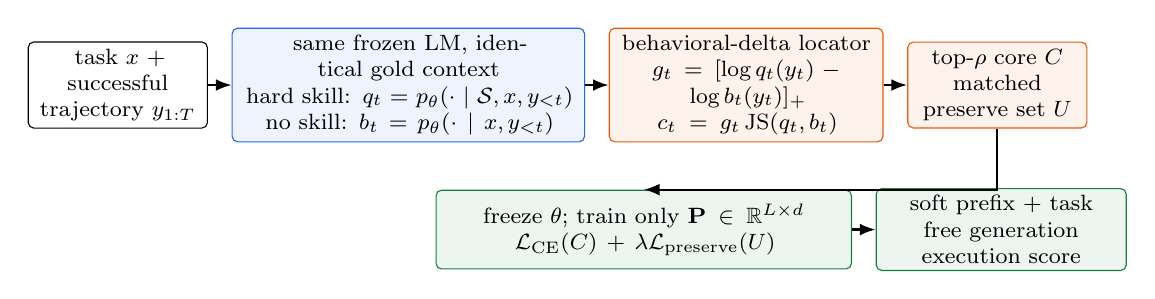
\begin{tikzpicture}[
  font=\footnotesize,
  node distance=6mm and 3mm,
  box/.style={draw,rounded corners=2pt,align=center,minimum height=10mm,inner sep=2.5pt},
  arr/.style={-{Latex[length=2mm]},thick},
  teacher/.style={box,fill=skillblue!8,draw=skillblue},
  student/.style={box,fill=skillgreen!8,draw=skillgreen},
  score/.style={box,fill=skillorange!8,draw=skillorange}
]
\node[box,text width=21mm] (data) {task $x$ + successful trajectory $y_{1:T}$};
\node[teacher,right=of data,text width=43mm] (paired) {same frozen LM, identical gold context\\hard skill: $q_t=p_\theta(\cdot\mid \skill,x,y_{<t})$\\no skill: $b_t=p_\theta(\cdot\mid x,y_{<t})$};
\node[score,right=of paired,text width=33mm] (locator) {behavioral-delta locator\\$g_t=[\log q_t(y_t)-\log b_t(y_t)]_+$\\$c_t=g_t\,\mathrm{JS}(q_t,b_t)$};
\node[score,right=of locator,text width=21mm] (select) {top-$\rho$ core $C$\\matched preserve set $U$};
\node[student,below=of locator,xshift=-13mm,text width=51mm] (train) {freeze $\theta$; train only $\prefix\in\mathbb{R}^{L\times d}$\\$\mathcal{L}_{\rm CE}(C)+\lambda\mathcal{L}_{\rm preserve}(U)$};
\node[student,right=of train,text width=30mm] (eval) {soft prefix + task\\free generation\\execution score};
\draw[arr] (data) -- (paired);
\draw[arr] (paired) -- (locator);
\draw[arr] (locator) -- (select);
\draw[arr] (select.south) |- (train.north);
\draw[arr] (train) -- (eval);
\end{tikzpicture}
\caption{\method separates \emph{where the hard skill changes behavior} from \emph{what the soft prefix must learn}.  The full-vocabulary distributions are used to locate a sparse core; current main training uses hard next-token targets on that core and a no-skill Top-64-plus-residual KL on unselected positions.  Only the soft-prefix embeddings are updated.}
\label{fig:overview}
\end{figure*}


\section{Related Work}

\paragraph{Parameter-efficient and prompt-based adaptation.}
Prefix tuning prepends learned continuous states throughout the Transformer~\citep{li2021prefix}, while prompt tuning optimizes input embeddings and becomes competitive as model scale grows~\citep{lester2021prompt}.  P-Tuning v2 extends deep prompts across scales and tasks~\citep{liu2022ptuningv2}; SPoT transfers prompts across tasks~\citep{vu2022spot}; residual prompt tuning improves optimization through a reparameterized residual path~\citep{razdaibiedina2023residual}; and InfoPrompt regularizes soft prompts using mutual-information objectives~\citep{wu2023infoprompt}.  LoRA instead learns low-rank weight updates~\citep{hu2022lora}.  Our setting is stricter: the model weights are frozen, only eight input embeddings are trainable, and the target is behavior induced by a long textual skill.

\paragraph{Context and prompt compression.}
Gist tokens learn to compress prompts into a small set of activations~\citep{mu2023gist}; AutoCompressors recursively summarize long contexts into soft memory~\citep{chevalier2023autocompressors}.  LLMLingua and its successors compress prompts by removing or reordering less informative discrete tokens~\citep{jiang2023llmlingua,jiang2024longllmlingua,pan2024llmlingua2}, while MEND learns a compact encoding for demonstrations~\citep{li2024mend}.  These methods primarily compress the input or demonstrations themselves.  \softskill instead learns from successful agent trajectories~\citep{tao2026softskill}.  On-policy context distillation optimizes a weight-updated student on its own trajectories against a privileged-context teacher~\citep{ye2026opcd}; this directly addresses the state mismatch that our frozen-prefix experiments expose, but changes many more parameters.  \method is an off-policy, parameter-efficient counterpart: it first identifies the hard skill's behavioral delta on verified trajectories.

\paragraph{Distillation and token selection.}
Knowledge distillation transfers teacher distributions to a student~\citep{hinton2015distilling}, with sequence-level KD using generated targets~\citep{kim2016sequence}.  For generative models, reverse-KL and on-policy formulations can better match the student's sampling distribution~\citep{gu2024minillm,agarwal2024gkd}.  Selective KD has been studied at the example and token levels~\citep{wang2021selective,tavor2026rethinking}; very recent work jointly adapts token selection and privileged teacher context to student capacity~\citep{yang2026usd}.  KFD is especially close in scoring tokens by divergence between a teacher and a related base model~\citep{yuce2026kfd}; Delta-KD similarly transfers the distributional shift from a raw to a fine-tuned teacher~\citep{cao2025delta}.  The distinction is the object being compressed: our teacher and reference are the \emph{same frozen agent} under hard-skill and no-skill contexts, and the only student parameters are an input prefix.  We further pair selective learning with an explicit clean-behavior preservation set and evaluate long-horizon executable generation rather than next-token accuracy alone.

\paragraph{Agent skills and prompt optimization.}
ReAct interleaves reasoning and action for language agents~\citep{yao2023react}, and AgentTuning studies instruction tuning over agent trajectories~\citep{zeng2024agenttuning}.  Natural-language prompts can be optimized using textual gradients or model-generated search directions~\citep{pryzant2023protegi,yang2024opro,yuksekgonul2024textgrad}; SkillOpt discovers reusable textual skills from successful rollouts~\citep{guo2026skillopt}.  Our work begins after a textual skill and successful trajectories exist and asks what portion of their induced behavior an extremely small continuous prefix can retain.

\section{Selective Behavioral Compression}
\label{sec:method}

\subsection{Problem setup}
Let $p_\theta$ be a frozen causal language model, $x$ an agent task, $\skill$ a textual skill, and $\traj=(y_1,\ldots,y_T)$ a successful trajectory.  We seek a soft prefix $\prefix_\phi\in\mathbb{R}^{L\times d}$ such that the frozen model conditioned on $(\prefix_\phi,x)$ reproduces the useful behavior of conditioning on $(\skill,x)$, without storing the hard skill in the inference context.  Only $Ld$ parameters are trainable.

For every target position we use the same teacher-forced state $(x,y_{<t})$ and compute
\begin{align}
q_t(v)&=p_\theta(v\mid \skill,x,y_{<t}), &
b_t(v)&=p_\theta(v\mid x,y_{<t}), \label{eq:teachers}\\
p^\phi_t(v)&=p_\theta(v\mid \prefix_\phi,x,y_{<t}).
\end{align}
The alignment is by construction: both distributions in Equation~\ref{eq:teachers} predict the next token of the \emph{same} tokenized successful trajectory.  Comparing independent generations would confound skill influence with divergent histories.

\subsection{Locating the behavioral delta}
We use two complementary signals.  The first is realized positive gain,
\begin{equation}
g_t=\left[\log q_t(y_t)-\log b_t(y_t)\right]_+,
\label{eq:gain}
\end{equation}
which asks whether the hard skill makes the gold next token more likely.  It is directional and trajectory-specific, but ignores redistributions among non-gold tokens.  The second is the full-distribution Jensen--Shannon divergence
\begin{equation}
j_t=\tfrac12\mathrm{KL}(q_t\Vert m_t)+\tfrac12\mathrm{KL}(b_t\Vert m_t),\qquad
m_t=\tfrac12(q_t+b_t).
\label{eq:js}
\end{equation}
Our Combined locator is
\begin{equation}
c_t=g_t\,j_t. \label{eq:combined}
\end{equation}
Multiplication favors states where the skill both moves the complete distribution and moves it in the direction realized by a successful trajectory.  For each trajectory, we select the highest-scoring $\rho$ fraction of eligible non-EOS tokens as core $C$; EOS is always supervised.  Stage-1 scoring uses exact full-vocabulary JS.  Top-64 probabilities and one residual-mass bucket are cached for later KL losses; they retain over 99.8\% probability mass on average in our data.

We diagnose sparsity by the concentration curve
\begin{equation}
\mathcal{C}(\rho)=\frac{\sum_{t\in\mathrm{Top}_\rho(g)}g_t}{\sum_{t=1}^T g_t}.
\end{equation}
High $\mathcal{C}(\rho)$ at small $\rho$ is a necessary, not sufficient, condition for selective compression: it says that the teacher effect is sparse on gold contexts, but not that the prefix can cause the same states during generation.

\subsection{Selective prefix objective}
The main implementation uses the hard trajectory token at selected positions rather than a dense teacher-distribution target:
\begin{equation}
\mathcal{L}_{\mathrm{core}}(\phi)=-\frac{1}{|C|}\sum_{t\in C}\log p^\phi_t(y_t).
\label{eq:core}
\end{equation}
Thus $q_t$ is used to discover \emph{where} supervision is attributable to the skill; the current main loss uses the successful token to specify \emph{what} to predict.  We reserve ``full Skill-KL'' for variants that explicitly optimize $\mathrm{KL}(q_t\Vert p_t^\phi)$.

Selective CE alone can change predictions everywhere because every prefix embedding affects all later activations.  We sample a matched-size preservation set $U$ outside both selectors in a paired comparison and anchor it to the no-skill reference:
\begin{equation}
\mathcal{L}_{\mathrm{pres}}(\phi)=\frac{1}{|U|}\sum_{t\in U}\mathrm{KL}\!\left(\tilde b_t\Vert\tilde p^\phi_t\right),
\label{eq:preserve}
\end{equation}
where $\tilde b_t$ and $\tilde p^\phi_t$ are categorical distributions over the 64 most probable reference tokens plus a single residual bucket.  The final loss is
\begin{equation}
\mathcal{L}=\mathcal{L}_{\mathrm{core}}+\lambda_{\mathrm{pres}}\mathcal{L}_{\mathrm{pres}},
\qquad \lambda_{\mathrm{pres}}=1.
\label{eq:loss}
\end{equation}
The prefix is initialized from the first $L$ token embeddings of the hard skill.  Base-model weights remain frozen throughout.

\subsection{Residual prefix boosting variants}
\label{sec:prcb}
We also test whether prefix coordinates can act as weak learners.  PRCB-v1--v4 repeatedly optimize overlapping coordinate blocks; v4-ES selects per-block steps on a held-out subset of training trajectories.  PRCB-v5 adds replay/retention and line-searches a block coefficient.  PRCB-v6 moves closer to functional boosting~\citep{friedman2001greedy}: each stage trains an independent prefix learner against the residual between hard-skill and current ensemble logits, freezes previous learners, line-searches a scalar $\alpha_s$, and rejects stages without global Skill-KL improvement.  These are diagnostic variants rather than the main method; their failures clarify why coordinate blocking is not equivalent to independent functional weak learners.

\section{Experimental Setup}
\label{sec:setup}

\paragraph{Benchmarks.}
Our main study uses SpreadsheetBench Verified~\citep{ma2024spreadsheetbench}, in which the model receives a natural-language spreadsheet-editing request and must produce Python whose execution yields the required workbook.  We use the repository's fixed 80/40/280 train/validation/test split.  A GPT-5.5 API service generated one hard-skill-conditioned trajectory per training task; execution filtering retained 61 successes (42/53 cell-level and 19/27 sheet-level tasks), containing 54,929 target tokens.  No failed trajectory is used for localization or training.  SearchQA is retained as a reproduction check of the inherited SoftSkill pipeline, not as evidence for our selective method.

\paragraph{Model and prefix.}
All SpreadsheetBench compression and free-generation results use the same local Qwen3.6-35B-A3B checkpoint~\citep{qwen2026qwen36}.  Its input embedding width is 2,048.  A length-8 prefix therefore contains 16,384 trainable values; all model parameters are frozen.  Unless stated otherwise, we use AdamW, learning rate $10^{-3}$, batch size 1 with two-step accumulation, BF16, gradient checkpointing, seed 1, and text initialization.  The core selector uses $\rho=5\%$, exact JS, and seed 1.  Main training runs one epoch and supervises 2,838 tokens including EOS, with 2,777 matched preservation positions.  The longest cached target is 3,647 tokens.

\paragraph{Baselines.}
\textbf{No Skill} evaluates the frozen model with only the task.  \textbf{Full-trajectory SoftSkill} trains the same length-8 prefix on every trajectory token.  \textbf{Random-5\%} replaces the locator with a matched random mask.  \textbf{Positive-5\%} ranks only by Equation~\ref{eq:gain}.  \textbf{Combined-5\%} uses Equation~\ref{eq:combined}.  Preservation variants add Equation~\ref{eq:preserve}.  Local-window variants expand each selected core by a fixed left/right radius.  Task-specific oracle experiments train one independent prefix per successful training task and then freely generate on that same task; they measure closure, not generalization.

\paragraph{Evaluation protocol.}
The final system receives a prefix and task, freely generates code greedily, executes it in the benchmark environment, and is successful only if the resulting workbook passes the task checker.  The main 280-task test comparison uses the same batch size 2, 8,192-token generation cap, frozen model revision, and execution environment.  We report exact paired McNemar tests; because one seed and one benchmark are available, confidence claims are deliberately limited.  Validation selection uses only the 40-task validation split.  The final Combined configuration is frozen before its single test run.  All task-specific oracle experiments explicitly set \texttt{test\_split\_accessed=false}.

\paragraph{Research questions.}
We ask: \textbf{RQ1}, is the hard skill's effect concentrated on a small fraction of successful-trajectory tokens?  \textbf{RQ2}, does selective training improve over full-trajectory CE?  \textbf{RQ3}, do full-distribution localization and no-skill preservation matter?  \textbf{RQ4}, why do improved teacher-forced objectives fail to translate monotonically to execution success?

\section{Results}
\label{sec:results}

\subsection{The skill effect is sparse on successful contexts}
Figure~\ref{fig:concentration} answers RQ1.  The top 1\% of positions capture 42.11\% of aggregate positive gain; the top 5\% capture 84.05\%; and the top 10\% capture 96.12\%.  All 61 trajectories individually satisfy $\mathcal{C}(10\%)\geq 0.6$ and $\mathcal{C}(20\%)\geq 0.8$.  Random selection closely tracks its nominal budget.  This strongly supports localization, although it does not establish controllability by a short prefix.

\begin{figure}[t]
\centering
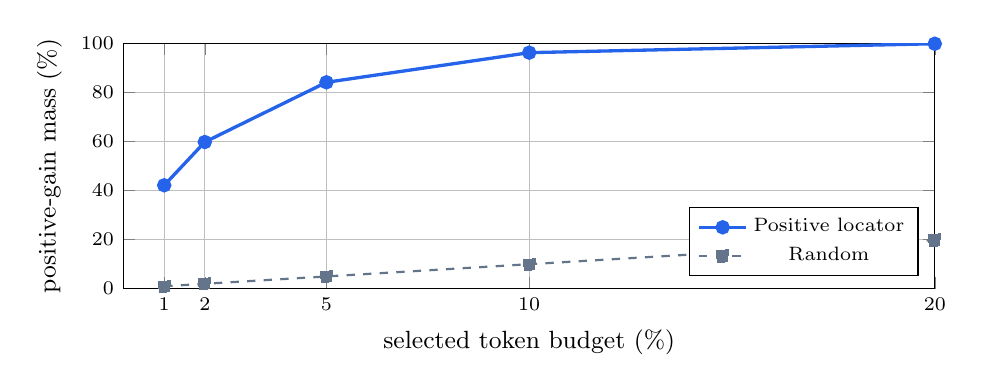
\begin{tikzpicture}
\begin{axis}[
    width=0.98\linewidth,
    height=4.7cm,
    xmin=0,xmax=20,
    ymin=0,ymax=100,
    xtick={1,2,5,10,20},
    ytick={0,20,40,60,80,100},
    xlabel={selected token budget (\%)},
    ylabel={positive-gain mass (\%)},
    grid=major,
    legend style={font=\scriptsize,at={(0.98,0.05)},anchor=south east},
    tick label style={font=\scriptsize},
    label style={font=\small}
]
\addplot[color=skillblue,very thick,mark=*] coordinates {(1,42.11) (2,59.72) (5,84.05) (10,96.12) (20,99.76)};
\addlegendentry{Positive locator}
\addplot[color=skillgray,dashed,thick,mark=square*] coordinates {(1,0.99) (2,1.99) (5,4.99) (10,9.97) (20,19.84)};
\addlegendentry{Random}
\end{axis}
\end{tikzpicture}
\caption{Aggregate concentration on 61 successful training trajectories.  Skill-induced positive gold-token gain is highly concentrated under teacher forcing.}
\label{fig:concentration}
\end{figure}


Positive and Combined select overlapping but non-identical cores (mean Jaccard 0.697).  At 5\%, Positive captures more realized gain (81.91\% vs.\ 76.23\%), whereas Combined captures more JS mass (50.61\% vs.\ 44.69\%) and combined-score mass (97.56\% vs.\ 95.90\%).  Full-distribution information therefore shifts capacity toward positions where the skill changes alternatives beyond the observed token.

\subsection{Selective compression improves over full-trajectory SoftSkill}

\begin{table}[t]
\caption{Matched SpreadsheetBench test results.  All methods use the same frozen Qwen checkpoint, 280 tasks, greedy decoding, batch size 2, and an 8,192-token cap.  $\Delta$ is relative to full-trajectory SoftSkill.}
\label{tab:test-main}
\centering
\small
\begin{tabular}{lrrr}
\toprule
Method & Solved & Success (\%) & $\Delta$ (pp) \\
\midrule
No Skill & 97/280 & 34.64 & +4.29 \\
Full-trajectory SoftSkill & 85/280 & 30.36 & -- \\
PRCB-v5 & 96/280 & 34.29 & +3.93 \\
\textbf{Combined-5\%+Preserve} & \textbf{101/280} & \textbf{36.07} & \textbf{+5.71} \\
\bottomrule
\end{tabular}
\end{table}


Table~\ref{tab:test-main} answers RQ2.  Combined-5\%+Preserve solves 101/280 test tasks, 16 more than full-trajectory SoftSkill.  The paired difference is significant under an exact McNemar test ($p=.0479$).  The improvement is entirely on cell-level tasks (61 vs.\ 45 of 193); both solve 40 of 87 sheet-level tasks.  This suggests that sparse instruction transfer helps local edits more than global workbook transformations.

The strongest conclusion is relative to the matched full-trajectory baseline, not the base model.  No Skill solves 97 tasks, and the four-task net advantage of Combined is not significant ($40$ Combined-only vs.\ $36$ no-skill-only, $p=.731$).  PRCB-v5 reaches 96/280 and likewise does not outperform No Skill.  Selectivity recovers the degradation introduced by indiscriminate trajectory fitting, but does not yet robustly add skill beyond the base model's existing competence.

\subsection{Validation ablations}

\begin{table*}[t]
\caption{SpreadsheetBench validation ablations (40 tasks).  ``Shared'' means Positive and Combined use the identical matched preservation indices.  Runs marked incomplete are excluded.}
\label{tab:validation}
\centering
\small
\begin{tabular}{lrrrrl}
\toprule
Training target & CE tokens & Coverage & Preserve & Epochs & Solved \\
\midrule
Full trajectory & 54,990 & 100.00\% & -- & 3 & 11/40 (27.5\%) \\
Random-5\% & 2,838 & 5.06\% & -- & 3 & 15/40 (37.5\%) \\
Random-5\% + KL & 2,838 & 5.06\% & 2,777 & 1 & 15/40 (37.5\%) \\
Positive-5\% + KL & 2,838 & 5.06\% & 2,777 & 1 & \textbf{18/40 (45.0\%)} \\
Positive-5\% + shared KL & 2,838 & 5.06\% & 2,777 & 1 & 10/40 (25.0\%) \\
Combined-5\% + shared KL & 2,838 & 5.06\% & 2,777 & 1 & 16/40 (40.0\%) \\
Positive window L2/R8 + KL & 19,424 & 35.25\% & 2,777 & 1 & 12/40 (30.0\%) \\
\bottomrule
\end{tabular}
\end{table*}


Table~\ref{tab:validation} answers RQ3.  With independent preservation sets, Positive-5\%+Preserve reaches 18/40 versus 15/40 for matched Random-5\%+Preserve.  In the stricter paired comparison with the same preservation indices, Combined improves over Positive (16/40 vs.\ 10/40), but the exact paired test is inconclusive ($p=.146$).  Expanding each Positive core by a left-2/right-8 window increases CE coverage from 5.06\% to 35.25\% yet reduces success to 12/40.  More local context is therefore not automatically better; it reintroduces abundant low-specificity targets and changes the loss scale.

\subsection{Task-specific capacity oracle}

To separate shared-prefix interference from representational limits, we train one prefix for each of the 61 successful training tasks and freely regenerate the \emph{same} task.  Combined core-only selection at 10\% solves 35/61 (57.38\%), compared with 32/61 (52.46\%) for the hard textual skill and 26/61 (42.62\%) for No Skill.  Five percent solves 28/61 and 20\% solves 33/61.  This is an oracle memorization/closure test, not held-out evidence, but it shows that an eight-token prefix can sometimes turn teacher-forced fitting into a successful rollout when cross-task interference is removed.  The non-monotonic 5/10/20\% curve also rules out ``insufficient token coverage'' as the sole explanation.

\section{Analysis: Why Better Token Fits Do Not Guarantee Better Agents}
\label{sec:analysis}

\paragraph{Gold-state localization versus generated-state control.}
Every locator score is computed on a verified trajectory prefix.  This is essential for causal comparability: hard-skill and no-skill distributions differ only in the skill.  During free generation, however, the prefix must first reproduce enough early structural decisions to remain on those states.  If it emits a different import, variable, workbook reference, or control-flow token, later training states become counterfactual.  This is the classical exposure-bias problem~\citep{bengio2015scheduled}; SpreadsheetBench amplifies it because semantic correctness is determined only after code execution.  Concentrated teacher effects can therefore coexist with weak rollout success.

\paragraph{The selected objective is local, while execution reward is structured.}
Equation~\ref{eq:combined} measures one-step distribution change, not a token's downstream causal effect.  A low-probability bracket or worksheet-selection call can determine whether hundreds of later tokens execute, while a high-JS lexical choice may have multiple semantically equivalent alternatives.  The multiplication $g_tj_t$ further suppresses positions where the hard skill changes the distribution but the cached gold token receives no positive gain.  Future locators should estimate downstream influence---for example, by teacher-forced suffix loss change, counterfactual execution, or on-policy visitation---without hand-designing fixed windows.

\paragraph{Why preservation helps but cannot solve the mismatch.}
The unselected KL prevents the prefix from arbitrarily degrading confident base behavior.  It is deliberately computed from a Top-64-plus-residual distribution rather than only the gold probability.  Yet it constrains only sampled gold states and only distributional drift.  It cannot guarantee syntactic invariants across a generated program, and it may oppose useful skill changes at unselected positions.  Its role is a trust region, not a proof of functional equivalence.

\paragraph{Why prefix-coordinate ``boosting'' mostly fails.}
Classic boosting adds weak learners in approximately independent function space~\citep{friedman2001greedy}.  Adjacent prefix vectors are not independent learners: through attention and every Transformer layer, updating one vector changes logits at nearly all subsequent tokens and changes the functional contribution of other vectors.  Consequently, PRCB-v1--v4 can reduce a block's monitored loss and still overwrite earlier behavior.  PRCB-v5's replay and line search reaches 18/40 validation tasks but only 96/280 test tasks.  PRCB-v6 creates independent full-length learners and combines their logits, but accepts only its first learner ($\alpha=.5$); the second stage obtains $\alpha=0$ even though 92.47\% of its selected core overlaps the previous core.  The residual remains large because the first learner has weak functional edge, not because the residual was computed without its prediction.  Distilling the ensemble back to one prefix does not improve validation; evaluating the undistilled ensemble also remains at 16/40.

\paragraph{What would materially change the optimization problem?}
The most promising next step is on-policy selective context distillation: sample student trajectories, query the hard-skill teacher on the exact student-visited states, select tokens subject to a capacity budget, and combine dense teacher KL with execution feedback.  This trades the clean causal interpretation of fixed gold contexts for coverage of the states encountered at inference.  A hybrid can retain verified gold anchors while adding student-state correction, related to on-policy context distillation~\citep{ye2026opcd} and generalized on-policy KD~\citep{agarwal2024gkd}.  This is a stronger intervention than another hand-chosen window or coordinate schedule.

\paragraph{Limitations.}
The current evidence is one model, one agent benchmark, one training seed, one teacher rollout per task, and a single final test evaluation.  The hard skill itself succeeds on only 61/80 training tasks, so the training set is success-conditioned.  Teacher generation uses a proprietary model, although trajectories are cached.  The main Combined configuration was chosen through validation comparisons, and the 280-task test was then used once; future changes must not reuse it for model selection.  Task-specific results are same-task oracles.  We report exact tests for paired outcomes but do not have multi-seed intervals.  These limitations prevent a broad state-of-the-art claim and define the experiments required before submission.

\section{Conclusion}

\method asks a simple question: if a textual skill changes a frozen model at only a small subset of successful-trajectory states, why train a tiny soft prefix on every token?  A paired hard-skill/no-skill locator finds that the effect is indeed sparse, and selective core training with clean-behavior preservation improves a matched full-trajectory SoftSkill baseline on SpreadsheetBench.  The same experiments also expose the boundary of the approach: local teacher-forced fit is not a reliable surrogate for free-running executable behavior, and coordinate-wise prefix updates do not inherit the independence assumptions of boosting.  We view the resulting method and negative results as a foundation for on-policy, capacity-aware skill compression rather than a finished solution to skill internalization.


\subsection*{AI use statement}
Generative AI tools were used during methodology exploration, implementation assistance, experiment analysis and interpretation, literature discovery, drafting, and \LaTeX{} preparation.  They were not used to autonomously decide benchmark labels or to alter execution outcomes.  This is a working draft: all AI-assisted prose, citations, claims, code references, and numerical results must be independently checked by the authors before submission.  The authors retain responsibility for the final content and artifacts.

\subsection*{Ethics statement}
The work studies compression of user-provided behavioral instructions into continuous prompts.  Such compression can reduce transparency because a soft prompt is not human-readable, and the same mechanism could conceal undesirable instructions.  We therefore recommend retaining the source skill, checksum, training provenance, and task-level audit logs whenever a learned prefix is distributed.  SpreadsheetBench contains synthetic office tasks and does not require human-subject data.  Teacher trajectories were generated through a commercial API; users reproducing them should follow the provider's terms and avoid uploading private spreadsheets.

\subsection*{Reproducibility statement}
The repository records data splits, prompt and skill hashes, cached successful trajectories, model revision, selection masks, Top-64 distribution summaries, checkpoints, per-task execution verdicts, and paired significance tests.  Appendix~\ref{app:repro} specifies commands and configurations; Appendix~\ref{app:results} reports all completed variants, including negative results.  The supplemental project includes code and manifests but excludes model weights, API credentials, and licensed benchmark assets.  An anonymous code URL will be inserted before submission.

\bibliography{references}
\bibliographystyle{iclr2027_conference}

\appendix
\section{Reproducibility Details}
\label{app:repro}

\subsection{Artifact map}
The source repository is organized around executable configurations rather than notebook-only experiments.  The primary entry points are:
\begin{itemize}
    \item \texttt{scripts/analyze\_selective\_distillation\_tokens.py}: two-pass teacher-forced scoring, exact JS, positive/Combined ranking, Top-64 caches, and concentration statistics;
    \item \texttt{scripts/prepare\_spreadsheetbench\_selective\_stage2.py}: matched core, random, window, coverage, and preservation manifests;
    \item \texttt{scripts/train\_soft\_prefix.py}: frozen-model prefix training and free-generation validation/test evaluation;
    \item \texttt{skillopt/softprefix/model.py}: masked selected-token CE and Top-$k$-plus-residual reference-to-prefix KL;
    \item \texttt{configs/spreadsheetbench/selective\_distillation\_stage1.yaml} and \texttt{selective\_distillation\_stage2.yaml}: main configurations;
    \item \texttt{docs/experiment\_results\_overview.md}: result provenance and command index.
\end{itemize}
API keys are loaded from local configuration and are intentionally excluded from the artifact.  Cached successful trajectory text is sufficient for the reported compression runs; regeneration is not required.

\subsection{Dataset construction and leakage controls}
The split contains 400 Verified tasks: 80 training, 40 validation, and 280 test.  The one-trajectory teacher cache is generated only for training tasks.  Execution succeeds on 61 tasks, and only those verified trajectories enter stage 1.  Locator thresholds are computed within training trajectories.  The 40-task validation set chooses among selectors and losses.  For the final test, the Combined checkpoint is frozen and hashed before generation.  The task-specific oracle reads only the 61 training tasks and records \texttt{test\_split\_accessed=false}.  PRCB-v4-ES further splits the 61 successful trajectories into 49 optimization and 12 teacher-forced monitoring trajectories; the monitor never backpropagates and validation execution is not used for early stopping.

\subsection{Optimization details}
The shared prefix has shape $8\times 2048$.  It is initialized with the embedding rows of the first eight tokens of the full hard skill.  Training uses learning rate $10^{-3}$, batch size 1, two gradient-accumulation steps, seed 1, BF16 model computation, and gradient checkpointing.  The main Combined run uses one epoch; its recorded total loss is 2.74714, consisting of selected CE 2.74054 and preservation KL 0.006605.  The wall-clock training time was 1,152.3 seconds in the recorded environment.  Generation is greedy.  Formal test runs use batch size 2 and \texttt{max\_new\_tokens=8192}; an earlier Positive diagnostic used batch size 8 and 4,096 tokens and is excluded from matched primary comparisons.

\subsection{Top-64-plus-residual KL}
For reference distribution $r$ and student $p$, let $K$ be the 64 highest-probability reference token IDs.  The cached categorical distribution is
\begin{equation}
\tilde r = \big(r(v_1),\ldots,r(v_{64}),1-\sum_{v\in K}r(v)\big).
\end{equation}
At training time the student probabilities on the same IDs and its complementary mass form $\tilde p$.  We compute $\mathrm{KL}(\tilde r\Vert\tilde p)$.  Mean cached mass is 99.859\% for hard-skill and 99.829\% for no-skill distributions, so the residual bucket is small but not discarded.

\section{Algorithm}
\label{app:algorithm}

\begin{figure}[h]
\small
\begin{minipage}{0.96\linewidth}
\textbf{Algorithm 1: Combined selective behavioral compression}
\begin{enumerate}
    \item For each successful $(x,\skill,y_{1:T})$, tokenize the target once.
    \item For each position $t$, run the frozen model on $(\skill,x,y_{<t})$ and $(x,y_{<t})$; compute $g_t$ by Eq.~\ref{eq:gain}, exact $j_t$ by Eq.~\ref{eq:js}, and $c_t=g_tj_t$.
    \item Select the top $\rho T$ eligible positions by $c_t$ as $C$; always include EOS.  Sample a same-budget set $U$ from positions outside the selectors being compared.
    \item Cache no-skill Top-64 token IDs, their log probabilities, and residual log mass for $U$.
    \item Initialize $\prefix_\phi$ from the first $L$ hard-skill token embeddings.  Freeze $\theta$.
    \item Minimize Eq.~\ref{eq:loss} over $\phi$ only.  Select the checkpoint on validation tasks, freeze it, and evaluate by task-conditioned free generation and workbook execution.
\end{enumerate}
\end{minipage}
\end{figure}

\section{Complete Locator Statistics}
\label{app:locator}

\begin{table}[h]
\caption{Positive-gain concentration across 61 successful training trajectories.  ``Aggregate'' pools gain mass; ``trajectory mean'' averages per-trajectory capture.}
\centering
\small
\begin{tabular}{rrrr}
\toprule
Top budget & Aggregate & Trajectory mean & Random \\
\midrule
1\%  & 42.11\% & 41.97\% & 0.99\% \\
2\%  & 59.72\% & 59.13\% & 1.99\% \\
5\%  & 84.05\% & 82.99\% & 4.99\% \\
10\% & 96.12\% & 95.42\% & 9.97\% \\
20\% & 99.76\% & 99.62\% & 19.84\% \\
\bottomrule
\end{tabular}
\end{table}

\begin{table}[h]
\caption{Top-5\% locator comparison.  Each selector has the same position budget.}
\centering
\small
\begin{tabular}{lrrr}
\toprule
Selector & Positive-gain mass & JS mass & Combined-score mass \\
\midrule
Positive gain & 81.91\% & 44.69\% & 95.90\% \\
Combined & 76.23\% & 50.61\% & 97.56\% \\
\bottomrule
\end{tabular}
\end{table}

\clearpage
\section{Complete SpreadsheetBench Results}
\label{app:results}

\subsection{Early and selective stage-2 runs}

\begin{table}[h]
\caption{Completed shared-prefix validation runs.  Results with different epochs or preservation sampling should not be treated as single-factor comparisons.}
\centering
\scriptsize
\begin{tabular}{lrrrr}
\toprule
Variant & CE positions & Preserve & Epoch & Success \\
\midrule
Full CE & 54,990 & 0 & 3 & 11/40 \\
Random-5 core & 2,838 & 0 & 3 & 15/40 \\
Positive-5 core & 2,838 & 0 & 2/3 & 13/40 (incomplete) \\
Random-5 core + independent KL & 2,838 & 2,777 & 1 & 15/40 \\
Positive-5 core + independent KL & 2,838 & 2,777 & 1 & 18/40 \\
Positive L2/R8 + independent KL & 19,424 & 2,777 & 1 & 12/40 \\
Positive-5 core + shared KL & 2,838 & 2,777 & 1 & 10/40 \\
Combined-5 core + shared KL & 2,838 & 2,777 & 1 & 16/40 \\
\bottomrule
\end{tabular}
\end{table}

\FloatBarrier
\subsection{PRCB variants}

\begin{table}[h]
\caption{Residual/block prefix experiments on the 40-task validation split.  Window indices denote trained prefix rows.}
\centering
\scriptsize
\begin{tabular}{p{3.2cm}p{6.7cm}rr}
\toprule
Variant & Schedule or defining change & Steps & Success \\
\midrule
Warm Combined & Starting checkpoint & -- & 16/40 \\
PRCB-v1 & Gradient-probed row pairs & 32 total & 14/40 \\
PRCB-v2 tail-to-head & $67\!\rightarrow\!45\!\rightarrow\!23\!\rightarrow\!01$ & 32 total & 11/40 \\
PRCB-v2 head-to-tail & $01\!\rightarrow\!23\!\rightarrow\!45\!\rightarrow\!67$ & 32 total & 15/40 \\
PRCB-v3 & Gold-context residual locator + margin & 32 total & 16/40 \\
PRCB-v4 & Overlap $01\!\rightarrow\!12\!\rightarrow\!\cdots\!\rightarrow\!67$ & 32 total & 16/40 \\
PRCB-v4-ES (width 2) & 49 train/12 monitor, rollback & 104 total & 14/40 \\
PRCB-v4-ES (width 5) & complete $01234,12345,23456,34567$ & 46 total & 13/40 \\
PRCB-v5 & replay/retention + coefficient line search & 74 total & \textbf{18/40} \\
PRCB-v6 & independent full-length functional learners & 28 total & 16/40 \\
PRCB-v6 low-rank & rank 2; 4,112/16,384 learner parameters & 18 total & 16/40 \\
\bottomrule
\end{tabular}
\end{table}

\FloatBarrier
In PRCB-v6, stage 1 improves global Skill-KL by 2.80\% and is accepted with $\alpha_1=0.5$.  Stage 2 is rejected with $\alpha_2=0$.  Its new core overlaps 2,568 of 2,777 previous positions (92.47\%).  The undistilled ensemble and the student distilled back to one prefix both solve 16/40, so final prefix distillation is not the primary failure.

\subsection{Paired test details}

For Combined versus full-trajectory SoftSkill, the net gain is 16 tasks and the exact McNemar $p$-value is .0479.  For Combined versus No Skill, 40 tasks are Combined-only and 36 are No-Skill-only, giving $p=.731$.  For PRCB-v5 versus SoftSkill, the exact paired $p$-value is .169.  These values are computed from per-task execution verdicts, not from unpaired proportions.

\subsection{Task-specific oracle}

\begin{table}[h]
\caption{Same-task oracle on the 61 successful training tasks.  Each row trains a separate length-8 prefix for 32 optimizer steps and evaluates it by free generation on its own task.  These numbers are not held-out generalization.}
\centering
\small
\begin{tabular}{lrrr}
\toprule
Condition & Success & Rate & Mean core Skill-KL closure \\
\midrule
No Skill & 26/61 & 42.62\% & -- \\
Hard Skill & 32/61 & 52.46\% & -- \\
Combined core-only 5\% & 28/61 & 45.90\% & 62.18\% \\
Combined core-only 10\% & \textbf{35/61} & \textbf{57.38\%} & 56.86\% \\
Combined core-only 20\% & 33/61 & 54.10\% & 50.74\% \\
\bottomrule
\end{tabular}
\end{table}

The closure metric is
\begin{equation}
\mathrm{closure}=1-
\frac{\mathrm{KL}(q_t\Vert p_t^\phi)}{\mathrm{KL}(q_t\Vert b_t)},
\end{equation}
averaged over selected core states.  A value of 57\% means that the prefix closes 57\% of the hard-skill/no-skill KL gap on cached gold contexts; it is not an execution-success percentage.  The fact that 5\% obtains higher closure than 10\% while solving fewer tasks is direct evidence that this local metric is misaligned with rollout success.

\section{SearchQA Reproduction Check}
\label{app:searchqa}

Before SpreadsheetBench, we reproduced the inherited SearchQA pipeline with Qwen3.5-4B and a length-32 prefix.  For the best soft-prefix checkpoint, the repository's two evaluation metrics (named ``hard'' and ``soft'' scoring, not hard-prompt and soft-prompt conditions) are 76.56\% and 82.45\% on the 64-example validation set, and 77.14\% and 84.33\% on the 1,400-example test set.  Training loss decreases from 0.3103 to 0.2286 to 0.1951 over three epochs.  SearchQA outputs are predominantly short answers, so this check verifies the basic compression chain but not long-horizon agent execution.

\section{Command Templates}
\label{app:commands}

The following commands are written relative to the repository root.  Paths to the local model cache may be overridden through the YAML files or command-line configuration.

\paragraph{Stage-1 locator.}
\begin{verbatim}
python -u scripts/analyze_selective_distillation_tokens.py \
  --config configs/spreadsheetbench/selective_distillation_stage1.yaml
\end{verbatim}

\paragraph{Prepare selective manifests.}
\begin{verbatim}
python -u scripts/prepare_spreadsheetbench_selective_stage2.py \
  --stage1-root outputs/SpreadsheetBench_selective_stage1_qwen36_gpt55 \
  --out-dir outputs/SpreadsheetBench_selective_stage2_manifests \
  --seed 1
\end{verbatim}

\paragraph{Train the Combined shared-preservation prefix.}
\begin{verbatim}
CUDA_VISIBLE_DEVICES=0 python -u scripts/train_soft_prefix.py \
  --config configs/spreadsheetbench/selective_distillation_stage2.yaml \
  --out_root outputs/SpreadsheetBench_combined_train \
  --cfg-options \
    train.num_epochs=1 \
    soft_prefix.trajectory_examples_path=\
outputs/SpreadsheetBench_selective_stage2_manifests/\
combined_top0.05_core_shared_preserve.jsonl \
    soft_prefix.preservation_loss_weight=1.0 \
    evaluation.sel_env_num=40 \
    evaluation.test_env_num=0 \
    evaluation.eval_test=false
\end{verbatim}

\paragraph{Frozen 280-task evaluation.}
\begin{verbatim}
CUDA_VISIBLE_DEVICES=0 python -u scripts/train_soft_prefix.py \
  --config configs/spreadsheetbench/selective_distillation_stage2.yaml \
  --out_root outputs/SpreadsheetBench_combined_test280 \
  --cfg-options \
    train.num_epochs=0 \
    evaluation.sel_env_num=0 \
    evaluation.test_env_num=0 \
    evaluation.eval_test=true \
    env.checkpoint_eval_val=false \
    env.generation_batch_size=2 \
    soft_prefix.max_new_tokens=8192 \
    soft_prefix.checkpoint_path=/ABSOLUTE/PATH/best_prefix.pt
\end{verbatim}

The checkpoint checksum and exact output directory should be fixed before running the last command.  The repository documentation contains the hashes used for completed formal runs.

\section{Pre-Submission Experiment Checklist}
\label{app:todo}

This draft is complete as an account of the current repository, but a competitive final submission should add: (i) at least three training seeds for the main locator and preservation baselines; (ii) a second agent benchmark with executable or environment-based scoring; (iii) a matched hard-skill test run; (iv) a direct selected-position Skill-KL target ablation against selected hard CE; (v) on-policy student-state distillation; (vi) compute, peak-memory, and prefix-inference latency measurements; (vii) bootstrap confidence intervals over tasks; and (viii) qualitative program traces showing where Combined fixes or breaks the baseline.  These are intentionally listed rather than silently implied by the existing evidence.


\end{document}
